
% \begin{figure*}
% \centering
% \begin{subfigure}[b]{0.49\linewidth}
%     \centering
%     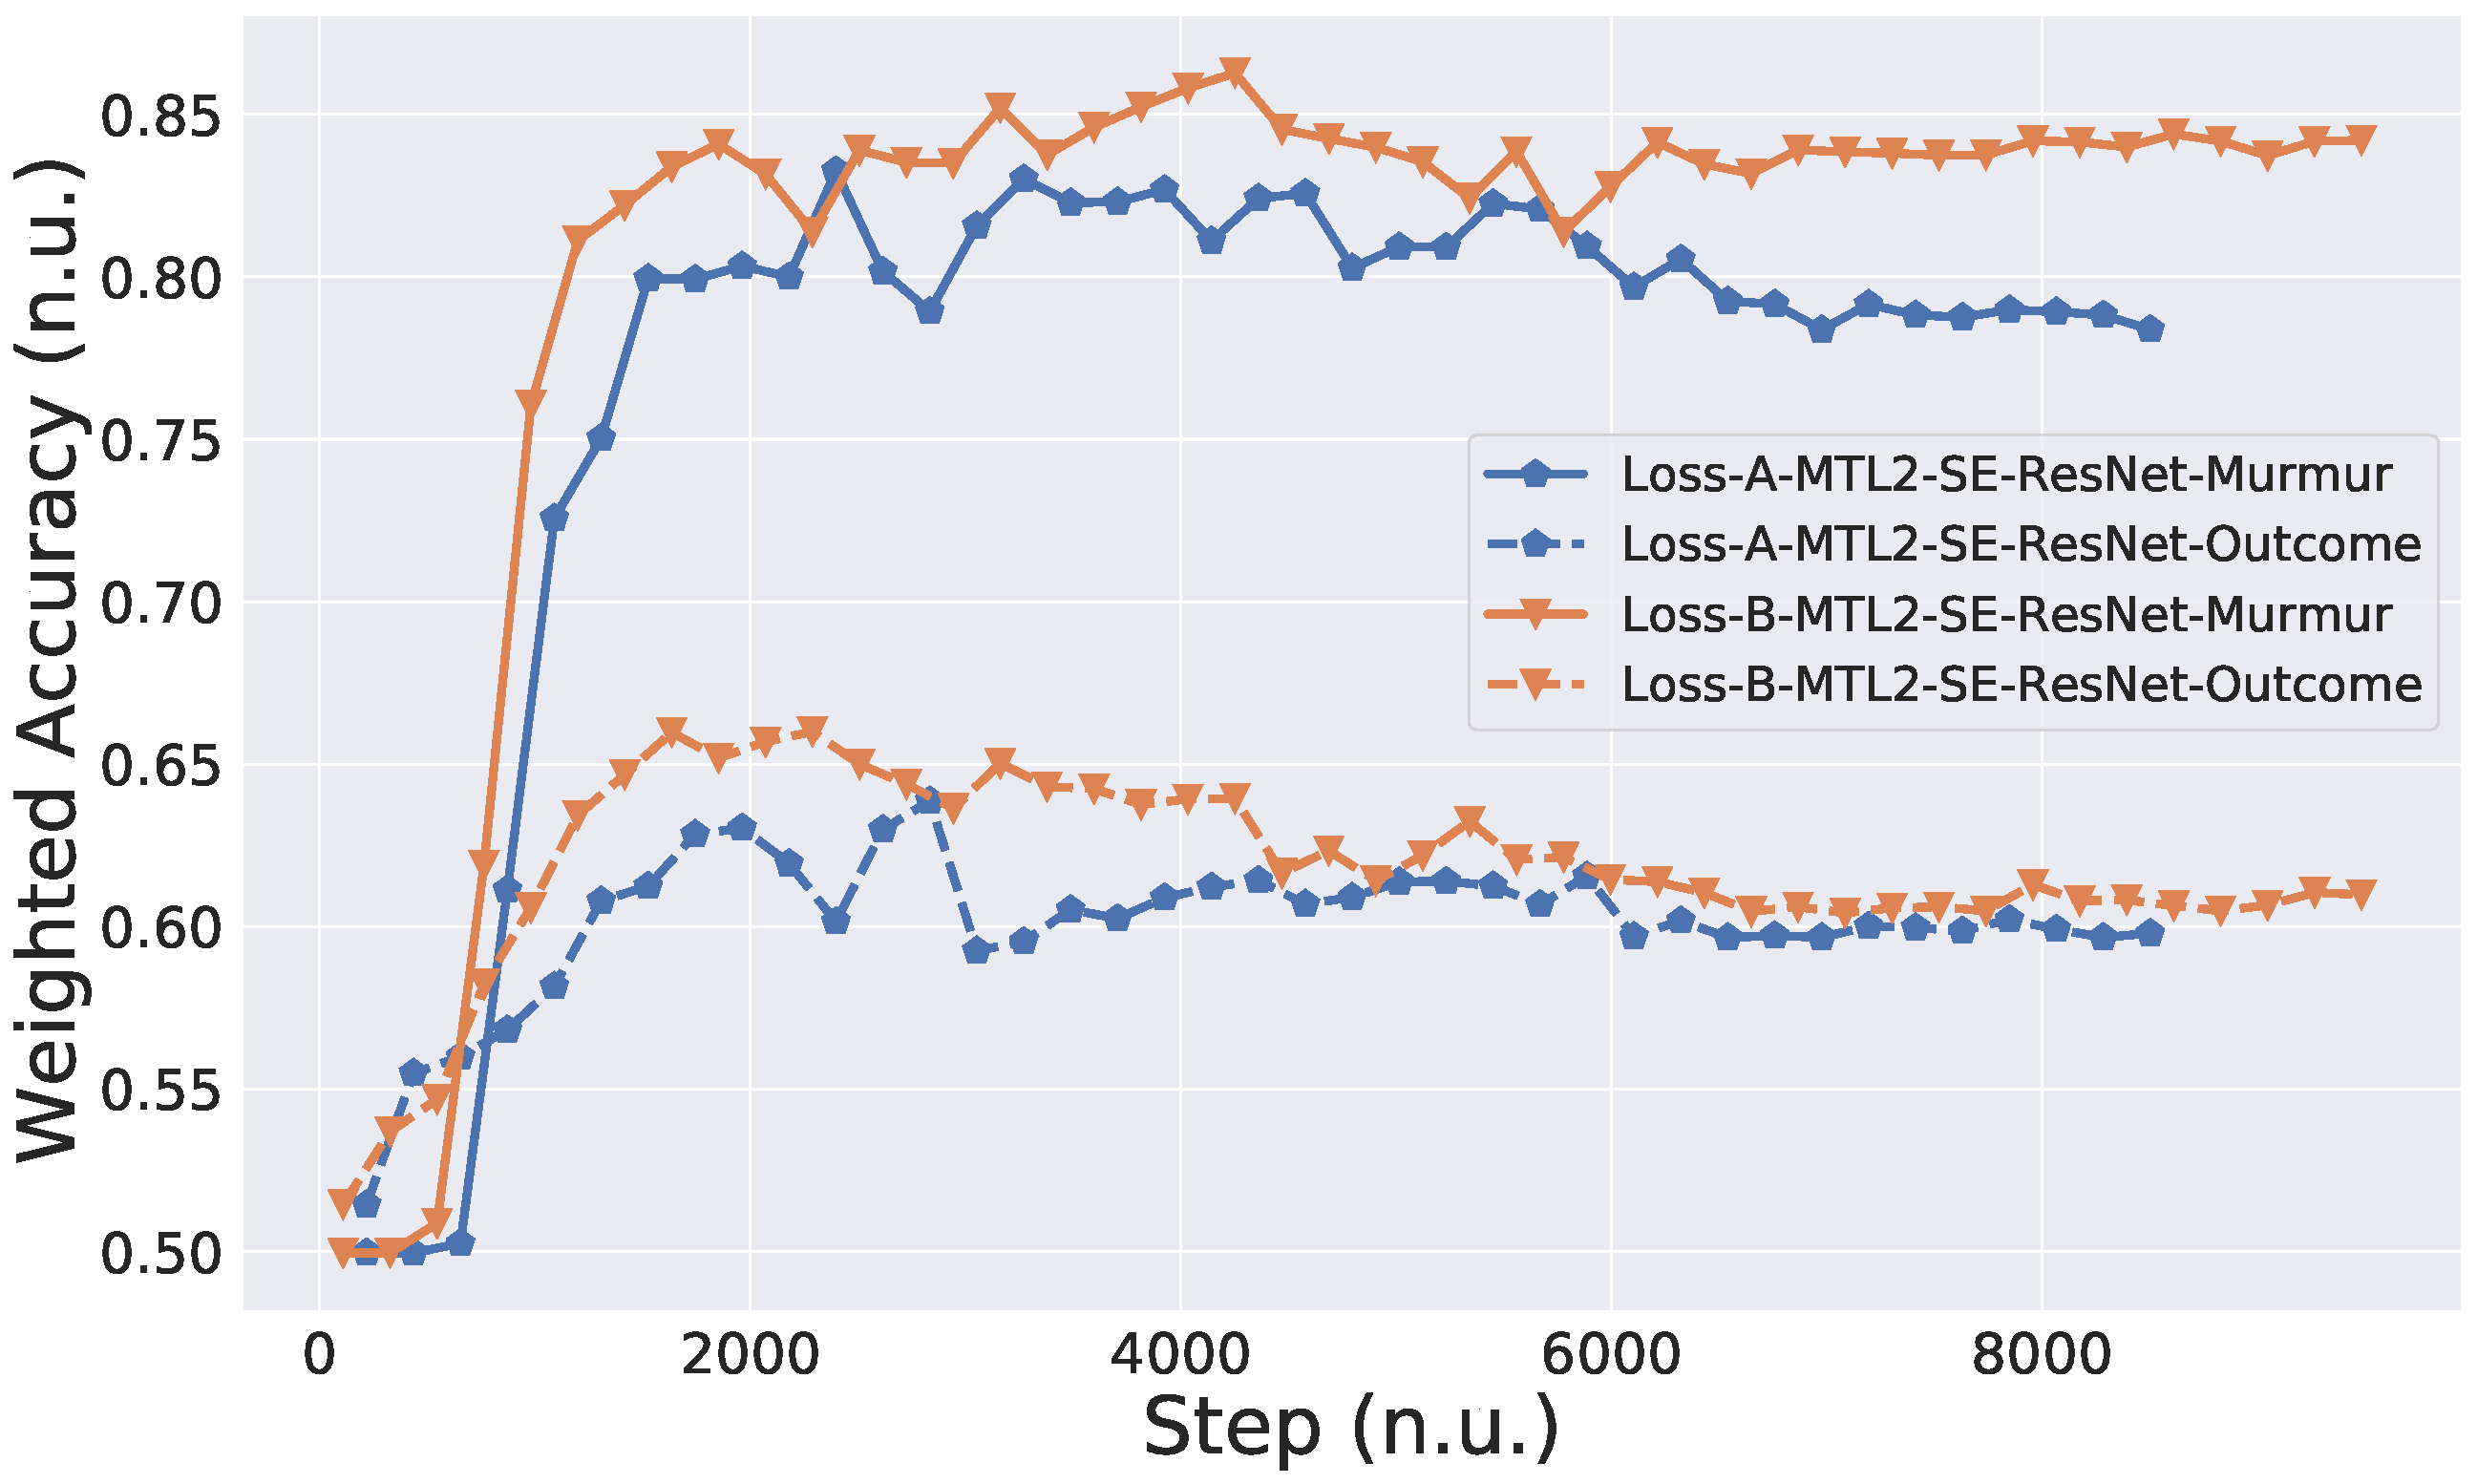
\includegraphics[width=\textwidth]{images/clf-se-resnet-lossA-vs-lossB.pdf}
%     \caption[]
%     {to write.}
%     \label{fig:clf-se-resnet-lossA-vs-lossB}
% \end{subfigure}
% \hfill
% \begin{subfigure}[b]{0.49\linewidth}
%     \centering
%     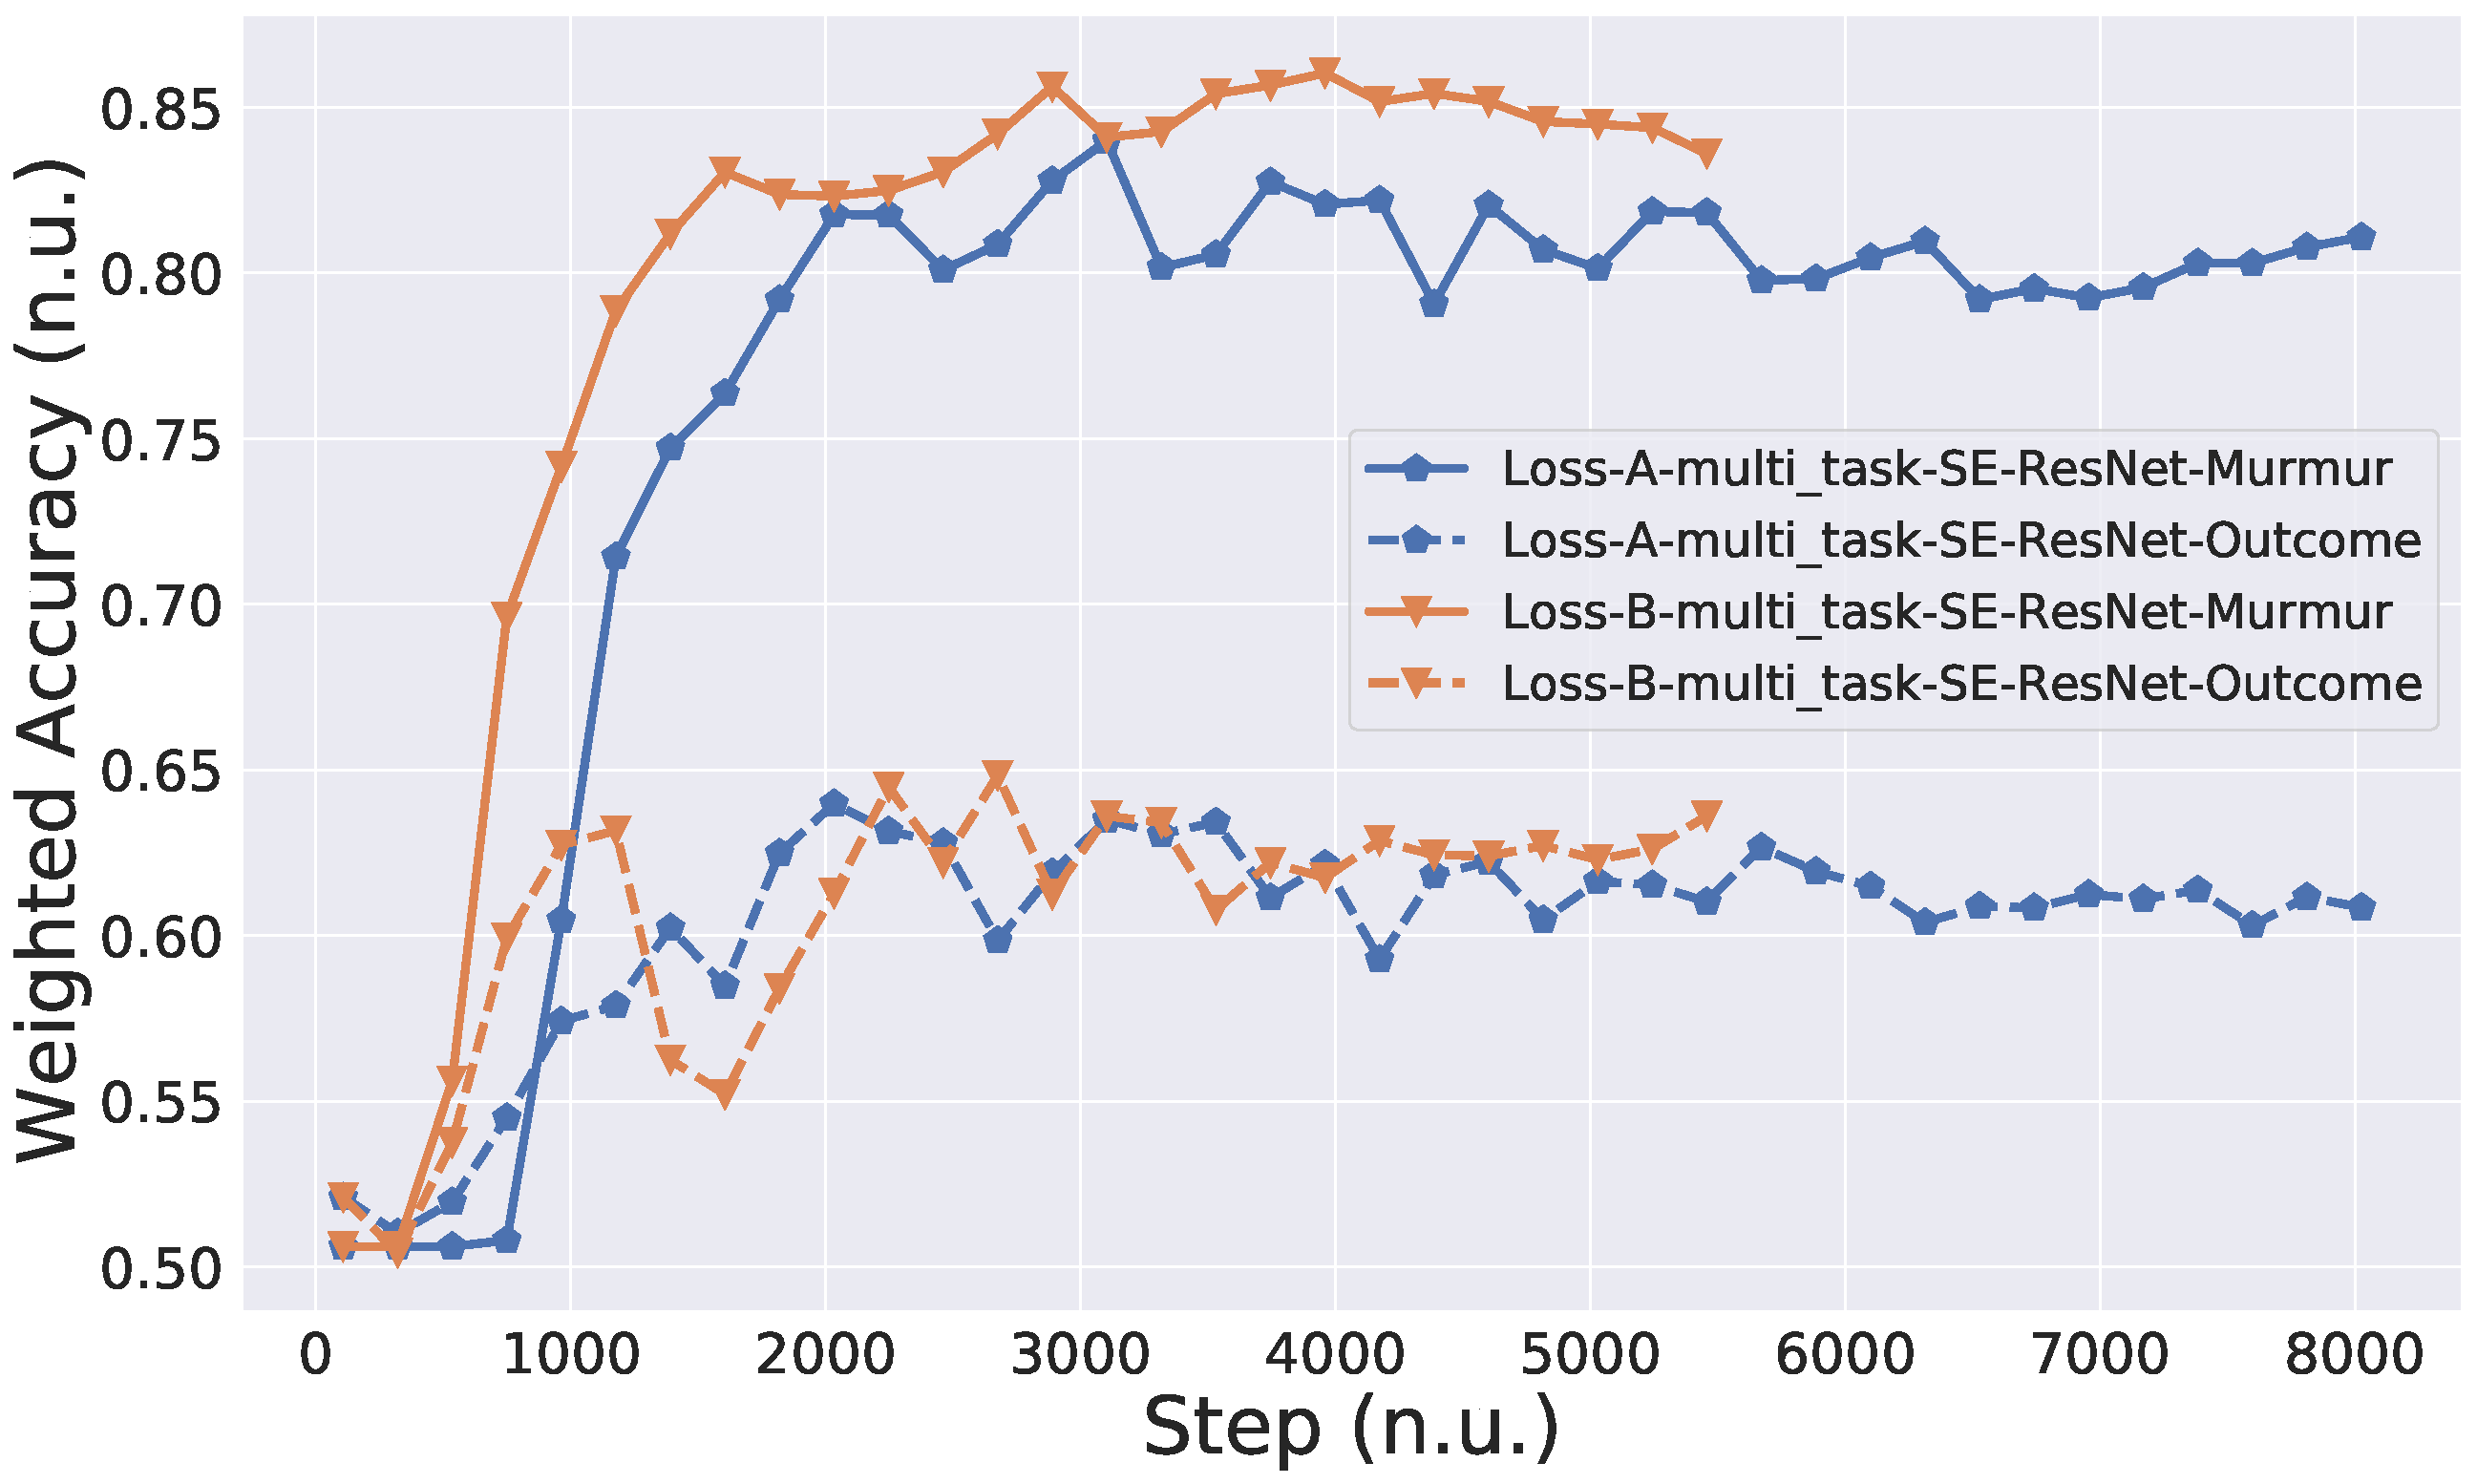
\includegraphics[width=\textwidth]{images/mtl-se-resnet-lossA-vs-lossB.pdf}
%     \caption[]
%     {to write}
%     \label{fig:mtl-se-resnet-lossA-vs-lossB.pdf}
% \end{subfigure}
% \caption[]
% {to write.}
% \label{fig:loss}
% \end{figure*}

\begin{figure}[!htp]
\centering
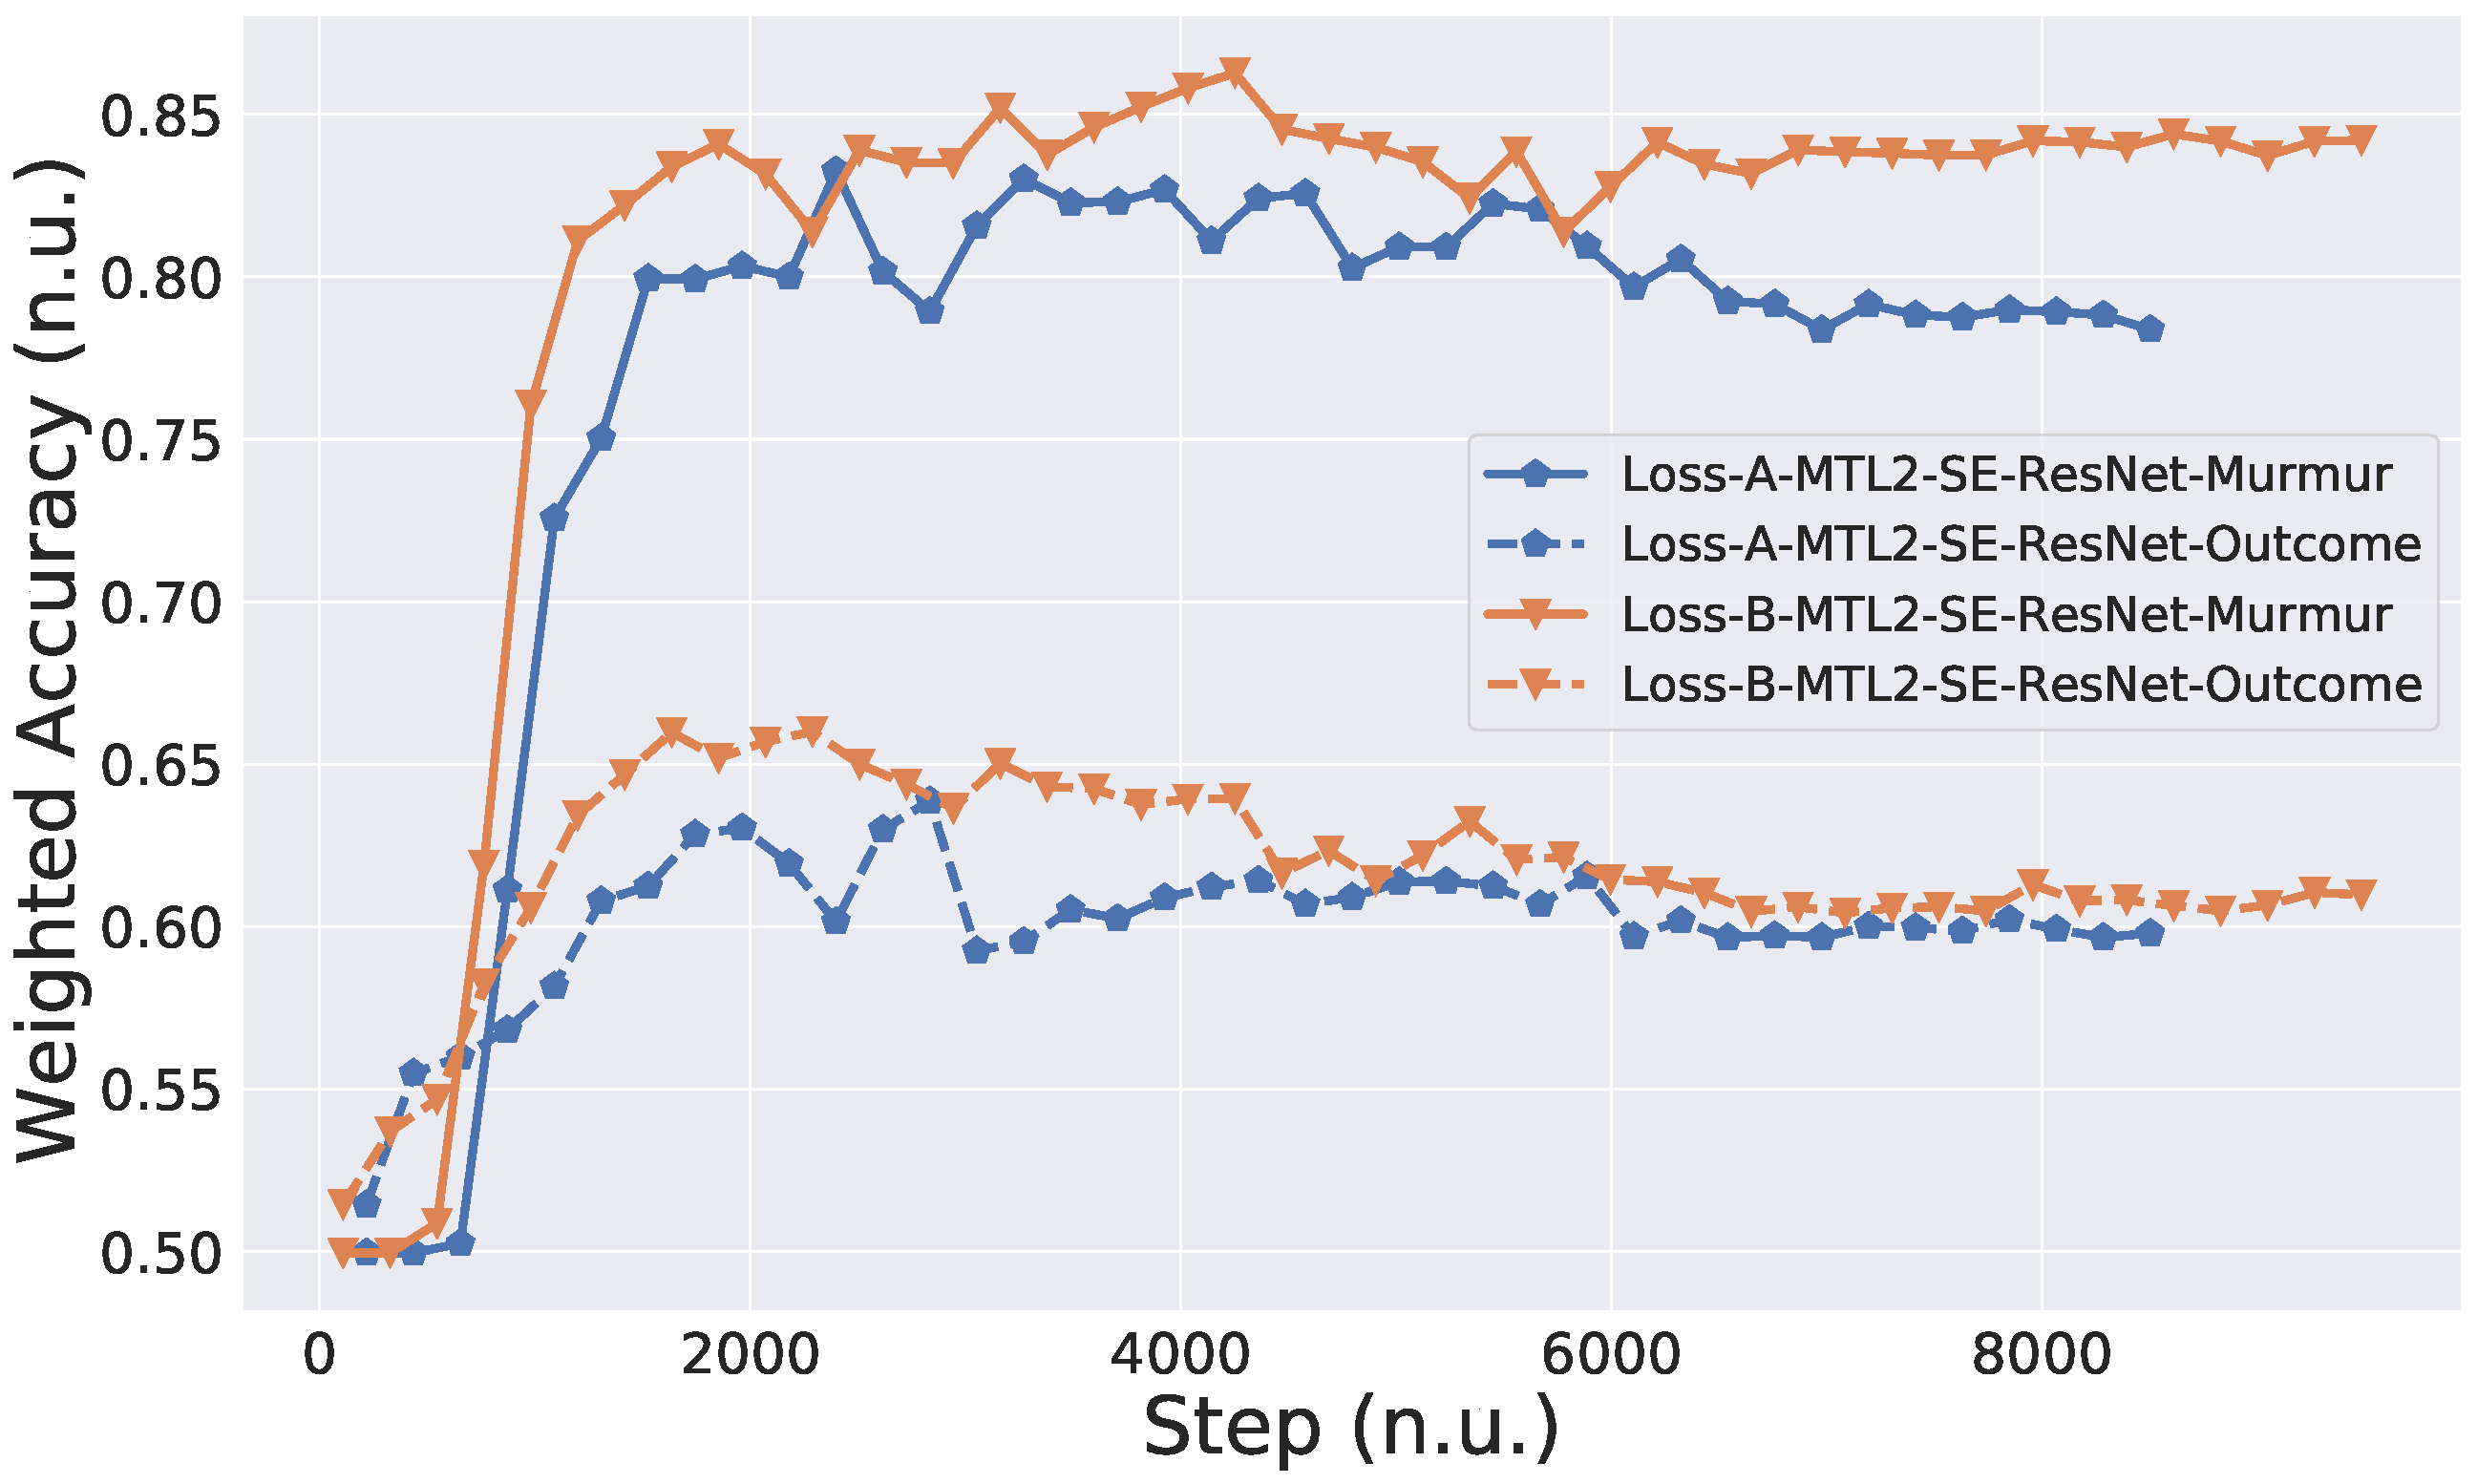
\includegraphics[width=\linewidth]{images/clf-se-resnet-lossA-vs-lossB.pdf}
\caption[]
{Experiments to compare the 2 loss functions. The model with 2 classification heads and with SE-ResNet as the backbone was used.}
\label{fig:clf-se-resnet-lossA-vs-lossB}
\end{figure}
